% https://es.overleaf.com/latex/templates/project-report/jpzczmpsdzwm

%%% Preamble
\documentclass[paper=leter, fontsize=11pt]{scrartcl}
\usepackage[utf8]{inputenc}
\usepackage[spanish,mexico]{babel}
\usepackage[T1]{fontenc}    % use 8-bit T1 fonts
\usepackage{lmodern}
\usepackage{hyperref}       % hyperlinks
\usepackage{lipsum}
\usepackage[square,numbers]{natbib}
\usepackage{enumitem}

\usepackage[protrusion=true,expansion=true]{microtype}	
\usepackage{amsmath,amsfonts,amsthm} % Math packages
\usepackage[pdftex]{graphicx}
\usepackage{url}
% https://tex.stackexchange.com/a/3785
\usepackage{breqn}
 
\usepackage{booktabs}
\usepackage[table,xcdraw]{xcolor}

\usepackage{tikz}
\usetikzlibrary{positioning,matrix, arrows.meta}

\usepackage{caption} 
\usepackage{subcaption}

\usepackage{multirow}

\usepackage{listings}
\lstdefinestyle{mystyle}{ 
    language=R,
    basicstyle=\ttfamily\footnotesize,
    breakatwhitespace=false,         
    breaklines=true,                 
    captionpos=b,                    
    keepspaces=true,                 
    numbers=left,                    
    numbersep=5pt,                  
    showspaces=false,                
    showstringspaces=false,
    showtabs=false,                  
    tabsize=2
}

\lstset{style=mystyle}
\renewcommand{\lstlistingname}{Código}


\selectlanguage{spanish}
\usepackage[spanish,onelanguage,ruled]{algorithm2e}


%%% Custom sectioning
\usepackage{sectsty}
\allsectionsfont{\centering \normalfont\scshape}


%%% Custom headers/footers (fancyhdr package)
\usepackage{fancyhdr}
\pagestyle{fancyplain}
\fancyhead{}											% No page header
\fancyfoot[L]{}											% Empty 
\fancyfoot[C]{}											% Empty
\fancyfoot[R]{\thepage}									% Pagenumbering
\renewcommand{\headrulewidth}{0pt}			% Remove header underlines
\renewcommand{\footrulewidth}{0pt}				% Remove footer underlines
\setlength{\headheight}{13.6pt}


%%% Equation and float numbering
%\numberwithin{equation}{section}		    % Equationnumbering: section.eq#
%\numberwithin{figure}{section}			    % Figurenumbering: section.fig#
%\numberwithin{table}{section}				% Tablenumbering: section.tab#

%\newtheorem{thm}{Theorem}
%\newtheorem{prop}{Proposition}
%\newtheorem{lemma}{Lemma}
\newtheorem{ex}{Exercise}

%%% Maketitle metadata
\newcommand{\horrule}[1]{\rule{\linewidth}{#1}} 	% Horizontal rule

%%% https://tex.stackexchange.com/a/118217
\usepackage{mathtools}
\DeclarePairedDelimiter\ceil{\lceil}{\rceil}
\DeclarePairedDelimiter\floor{\lfloor}{\rfloor}

\title{
		%\vspace{-1in} 	
		\usefont{OT1}{bch}{b}{n}
		\normalfont \normalsize \textsc{Posgrado de Ingeniería de Sistemas} \\ [25pt]
		\horrule{0.5pt} \\[0.4cm]
		\huge Ley de los grandes números \\
		\horrule{2pt} \\[0.5cm]
}
\author{
		\normalfont 								\normalsize
        Alberto Benavides\\[-3pt]		\normalsize
        \today
}
\date{}


%%% Begin document
\begin{document} 
\maketitle

\section{Introducción}

La ley de los grandes números afirma que mientras un experimento aleatorio se repita $n$ veces, el promedio de los resultados $\frac{X_1, X_2, \ldots, X_n}{n}$ de ese experimento se aproximará a su valor esperado $E(X)$ conforme $n$ se aproxime a $+\infty$.

Los ejemplos más usados para mostrar la ley de los grandes números consisten en lanzar una moneda al aire o la tirada de un dado de seis caras.

Para el lanzamiento de una moneda, el $E(X) = 0.5$. Los lenguajes computacionales permiten experimentar computacionalmente mediante la generación de valores pseudoaleatorios\footnote{https://es.wikipedia.org/wiki/Generador_de_n\%C3\%BAmeros_pseudoaleatorios}. En R\footnote{https://www.r-project.org/} se puede realizar un experimento que simule mil lanzamientos de monedas para, de ellos, calcular la media, con el procedimiento \texttt{mean(sample(0:1, 1000, replace=TRUE))}. Con una semilla fija \texttt{set.seed(33)}, se obtiene por resultado $0.507 \approx E(X)$. En este caso, el \texttt{0:1} simula los valores que puede tomar la variable aleatoria $X$: \texttt{0} para cara y \texttt{1} para cruz. 

En el caso de mil tiradas de un dado de seis caras, se puede simular con \texttt{mean(sample(1:6, 1000, replace=TRUE))}, donde el valor obtenido con la misma semilla es $3.554 \approx  E(X) = \frac{1 + 2 + 3 + 4 + 5 + 6}{6} = 3.5$.

Una representación gráfica de la parte en la que $n$ se aproxima a $+\infty$ consiste en graficar las medias conforme $n$ crece. Para el ejemplo de la tirada del dado de seis cara en la que se registran las tiradas en un rango $i \in [1, 10\ 000]$, se logra mediante el código \ref{dados}.

\begin{lstlisting}[caption={Medias experimentales de las tiradas de un dado de seis caras}, captionpos=t, label=dados]
  medias <- c()
  for (i in 1:10000){
      medias <- c(medias, mean(sample(1:6, i, replace=TRUE)))
  }
\end{lstlisting}

Las medias de cada $i$ número de experimentos se almacenan en una variable cuyos valores, mostrados en la figura \ref{fig:dados} (p. \pageref{fig:dados}), permite ver cómo converge al $E(X)$ el resultado de las medias conforme el número de repeticiones del experimento se hace más grande.

\begin{figure}
  \centering
  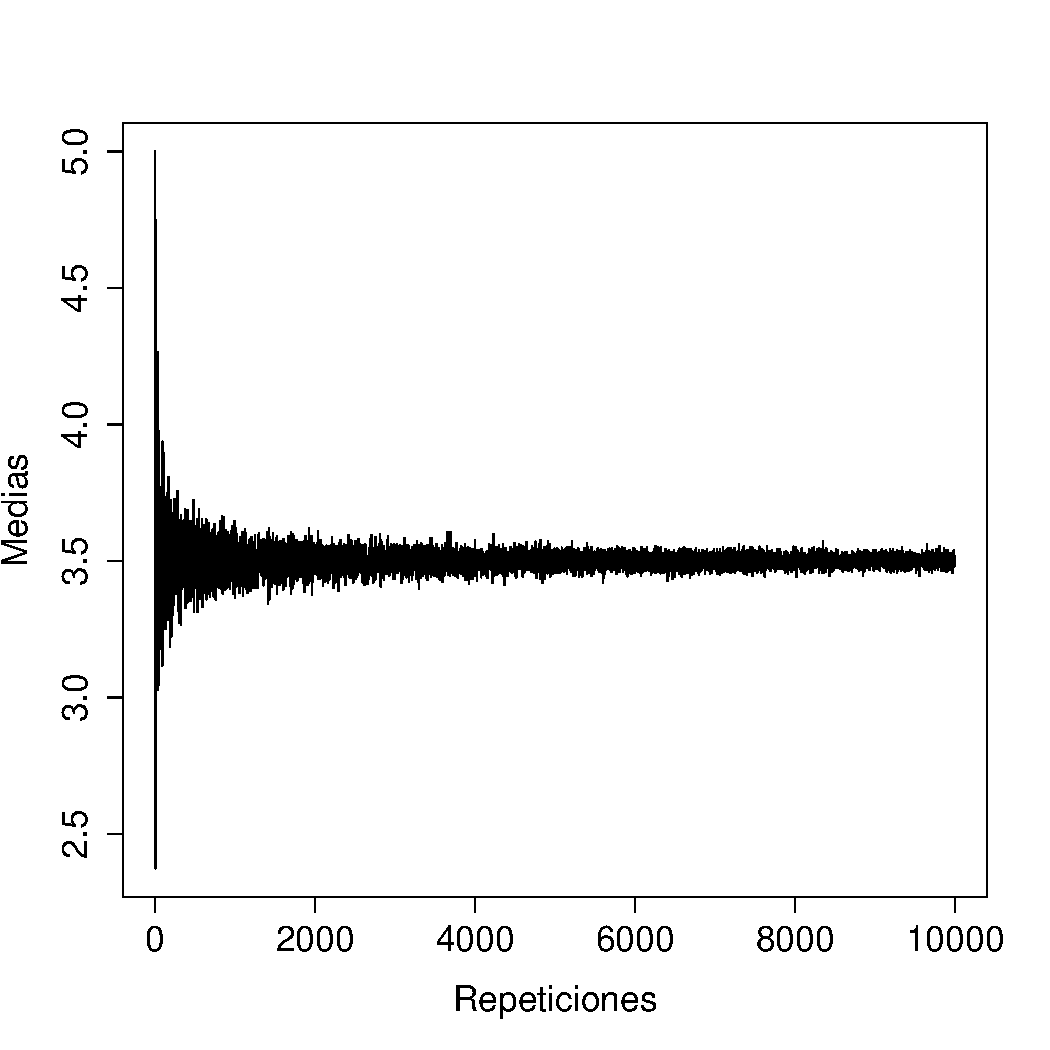
\includegraphics[width=0.8\textwidth]{dados.pdf}
\caption{Medias experimentales de distintas tiradas de dados.}
\label{fig:dados}
\end{figure}

\section{Problema}

Actualmente, investigo la relación que hay entre los contaminantes del aire y los reportes de enfermedades por parte de los centros de salud, estudio delimitado al Área Metropolitana de Monterrey durante el año 2017. Los datos de contaminantes para ese año se obtuvieron del Sistema Integral de Monitoreo Ambiental (SIMA) \cite{aireNL}. Un ejemplo de los datos obtenidos puede verse en la tabla \ref{tabla:amm} (p. \pageref{tabla:amm}), donde se constata que existen entre los datos la fecha en que fueron registrados, una de las trece estaciones que hizo el registro, los valores de ciertos contaminantes. Además, hay una columna llamada Válida, Elisa Schaeffer\footnote{https://elisa.dyndns-web.com/} agregó para diferenciar las mediciones inválidas conforme a lineamientos que el SIMA también proporcionó. Si la medición es válida, se asigna un valor de 1, mientras que si es inválida en alguno de los valores reportados, se le asigna un valor de 0.

\begin{table}
  \centering
  \caption{Muestra de mediciones capturadas por los sensores del área metropolitana de Monterrey.}
  \label{tabla:amm}
  \begin{tabular}{rccccc}
    \hline
  Fecha & Estación & CO & NO & $\ldots$ & Válida \\ 
    \hline
    19-Aug-16 16 & Centro & 0.43 & 1.90  & $\ldots$ & 1 \\ 
    23-Mar-97 0 & Sureste & 1.23 & 1.25  & $\ldots$ & 1 \\ 
    21-Oct-11 0 & Norte   & 2.16 & 40.00 & $\ldots$ & 1 \\ 
    \hline
  \end{tabular}
\end{table}

Uno de los problemas que se ha tenido con estos datos es la cantidad de errores en medición que presentan y una de las preguntas que se plantean por esta situación es qué estrategias se pueden implementar para mejorar la precisión de los sensores. En esta tarea se presenta una respuesta que utiliza la ley de los grandes números para encontrar un número de mediciones que se deberían hacer a partir de la media de valores inválidos registrados para saber si un cambio o reparación en los sensores mejora su certeza.

\section{Solución}

Los errores de medición detectados por Elisa Schaeffer se agruparon por año y estación de monitoreo, obteniendo por resultado registros como los que se muestran en la tabla \ref{tabla:agrupados} (p. \pageref{tabla:agrupados}).

\begin{table}[ht]
  \centering
  \caption{Cantidad de errores agrupados}
  \label{tabla:agrupados}
  \begin{tabular}{rcrr}
    \hline
    Año & Estación & Errores & Datos por grupo \\ 
    \hline
    1999 & Noroeste & 40 & 8760 \\ 
    2003 & Suroeste & 0 & 8760 \\ 
    2000 & Centro & 35 & 8784 \\ 
     \hline
  \end{tabular}
\end{table}

La estación con más errores de medición, con un total de $41.47\%$, es la Suroeste, cuya ubicación geográfica se muestra en la figura \ref{fig:so_geo} (p. \pageref{fig:so_geo}).

\begin{figure}
  \centering
  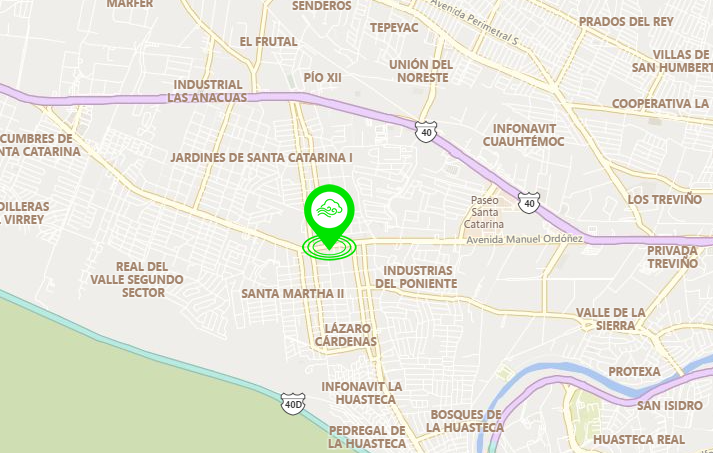
\includegraphics[width=0.8\textwidth]{so.png}
\caption{Mapa que muestra la ubicación de la estación de monitoreo Suroeste con un marcador de posición verde. Imagen obtenida de la página del SIMA\cite{aireNL}.}
\label{fig:so_geo}
\end{figure}

Análogo al ejemplo 4.3 descrito por \citet{Sedor2015}, se puede calcular la cantidad de mediciones que se deben hacer para saber, con un $95\%$ de confianza, que el porcentaje de errores de medición se mantiene. En el caso de la estación Suroeste, se sabe que la probabilidad de obtener una medición errónea es $\mu = 0.4147 = p$, de donde $\sigma^2 = p(1 - p) = 0.2427$. Ahora, se puede definir un error de medición $\epsilon = 0.02$, lo que quiere decir que se probará si una medida es errónea con probabilidad entre $[0.4147 - 0.02, 0.4147 + 0.02]$. Por la ley de los grandes números, se tiene que
$$P[|\bar{X} - \mu| > \epsilon] \leq \frac{\sigma^2}{n \epsilon^2},$$ 
al sustituir
$$P[|\bar{X} - 0.4147| > 0.02] \leq \frac{0.2427^2}{n (0.02)^2}.$$
Como se desea obtener un intervalo de confianza de $95\%$, entonces se debe cumplir
$$\frac{0.2427^2}{n (0.02)^2} = 0.05,$$
por lo que
$$n = \frac{0.2427^2}{(0.05) (0.02)^2} = 2945.1645 \approx 2945.$$

Así, se podría recomendar realizar $n = 2945$ mediciones y comparar el porcentaje de errores encontrados, para saber si alguna modificación en los sensores ha modificado la certeza de sus mediciones.
 
\bibliographystyle{mighelnat}
\bibliography{Biblio}

\end{document}